\documentclass[a4paper,12pt]{report}

\usepackage{alltt, fancyvrb, url}
\usepackage{graphicx}
\usepackage[utf8]{inputenc}
\usepackage{float}
\usepackage{hyperref}

% Questo commentalo se vuoi scrivere in inglese.
\usepackage[italian]{babel}

\usepackage[italian]{cleveref}

\title{Relazione Assignment-01 \\ per l'esame \\ ``Programmazione Concorrente e distribuita''}
\author{Rattini Emiliano\\Giosuè Giocondo Mainardi}

\date{\today}


\begin{document}

\maketitle

\tableofcontents

\chapter{Analisi}
% A brief analsysis of the problem, focusing in particular aspects that are relevant from concurrent point of view.
Il programma dei boid, ideato da Craig Reynolds nel 1986, modella un sistema in cui più entità, appunto i boid,
si muovono nello spazio modificando la propria traiettoria in base ai boid che hanno intorno ed a dei parametri definiti.
Considerado che ogni boid dovrà modificare la propria velocità, leggendo la posizione dei vicini, l'approccio migliore
sarà probabilmente quello di modificare prima tutte le velocità per poi aggiornare tutte le posizioni, ed infine
comunicarlo alla view.
Dal punto di vista concorrente, per ottimizzare il tempo di elaborazione delle velocità e delle posizioni, sarà
sicuramente conveniente suddividere il lavoro per più unità di calcolo, così da sfruttare appunto la concorrenza.
Ci sarà comunque quache differenza tra i 3 approcci implementati.

\chapter{Design}
% A description of the adopted design, the strategy and architecture.
Il design considerato non varia eccessivamente da versione a versione: ogni versione eredita da una superclasse che ha
i metodi comuni. Dalla versione sequenziale è stata cambiata la gestione del framerate, che viene calcolato da un counter
incrementato ad ogni fine calcolo di velocità e posizioni e comunicato alla view da un thread a parte.
Inoltre per rendere la view il più responsive possibile, si è gestita la parte di start, stop e resume attraverso dei
campi del model, di modo che il ciclo che aggiorna la view non andasse mai in wait.

\section{Multithreaded}
Nella versione multithreaded si è deciso di suddividere il carico di lavoro in un numero di thread pari al numero di processori
della macchina su cui gira il programma. Ogni thread aggiorna la velocità e la posizione della sua partizione di thread.
Per requisito, dovendo prima aggiornare tutte le velocità e poi successivamente tutte le posizione, si sono usate due barriere,
una per le velocità e una per le posizioni, cosicchè i thread si sincronizzino e svolgano tutti lo stesso compito.
Inoltre, come azione di rottura della seconda barriera, considerata come fine iterazione, si è aggiunto l'incremento del
counter di iterazioni per il calcolo del framerate.

\section{Executors}
Nella versione con l'executor framework la strategia cambia, poichè ragionando a task, il calcolo di un singolo boid
diventa un'unica unità di calcolo finita che viene delegata dallo stesso thread che aggiorna la view.
Considerando una dimensione a priori per le partizioni di boid, ognuna di esse viene assegnata ad un task per il calcolo
delle velocità e poi per quello delle posizioni. La sincronizzazione avviene attraverso i Future ritornati dall'Executor,
per i quali aspettiamo il completamento prima di passare al calcolo successivo. Alla fine del calcolo delle posizioni
viene aggiornato anche il counter di iterazioni per il framerate.

\section{Virtual threads}
Nella versione con i virtual threads l'approccio è un mix dei due precedenti poichè non considerando quanti thread
possiamo generare in base ai processori, ne generiamo tanti quanti le partizioni del nostro set di boid, come nella versione
executor. Però, non avendo i Future, come meccanismo di coordinazione abbiamo deciso di riusare le barriere, come appunto
nel caso dei Platform threads

\chapter{Comportamento}
% A description of the behaviour of the system using one or multiple Petri Nets, choosing the propor level of abstraction.

\chapter{Test di performance}
% Performance tests, to analyse and discuss the performance of the programs (for each version) compared to the sequential version

\chapter{Verifica con JPF}
% Verification of the program (a model of it) using JPF. For this point, only the Java multithreaded programming version may be considered.

\chapter{Esempi di utilizzo}
Esempio di immagine inserita sul posto.
\begin{figure}[h]
\centering{}
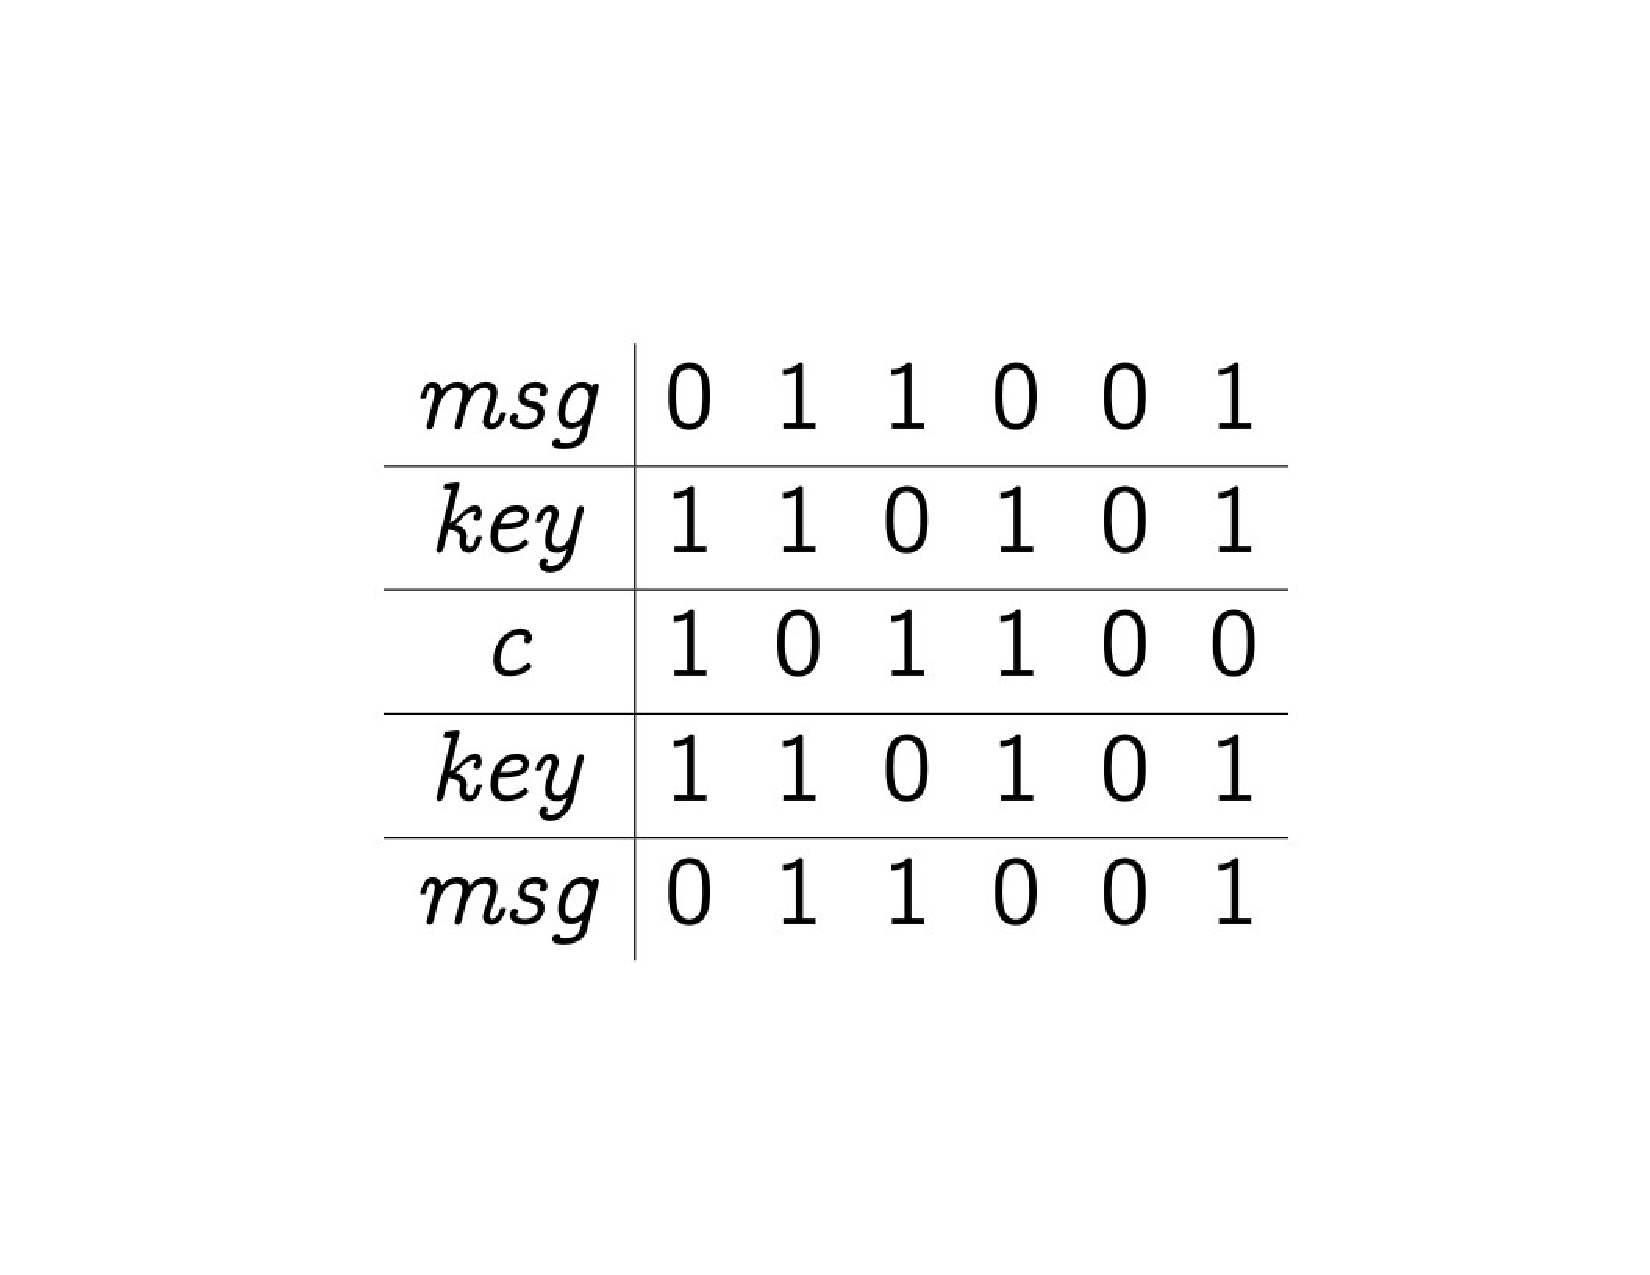
\includegraphics[width=\textwidth]{img/example_img.pdf}
\caption{L'interfaccia \texttt{GLaDOS}.}
\label{img:example}
\end{figure}

\paragraph{Paragrafo Risposta 1} Contenuto \textit{paragrafo}, con riferimento immagine
\Cref{img:example}: e anche \texttt{Scrittura unicode}.

Esempio di link
Permalink: \url{https://github.com/AlchemistSimulator/Alchemist/blob/d8a1799027d7d685569e15316a32e6394632ce71/alchemist-incarnation-protelis/src/main/java/it/unibo/alchemist/protelis/AlchemistExecutionContext.java#L141-L143}

% \appendix
% \chapter{Capitolo appendice 1}

% Contenuto.

% \chapter{Capitolo appendice 2}

% Contenuto.

\bibliographystyle{alpha}
\bibliography{report-template}

\end{document}
